\documentclass[../main.tex]{subfiles}
% !TEX root= ../main.tex

\begin{document}

\subsection{GPUs and Data Parallelism}

\begin{itemize}
	\item \textbf{Data Parallelism:} computation that does the same thing to lots of data
	\item Data-parallel programming often based on "outer-loop" parallelism, leaving the parallelism of the inner loop for instruction level parallelism
\end{itemize}

\begin{center}
	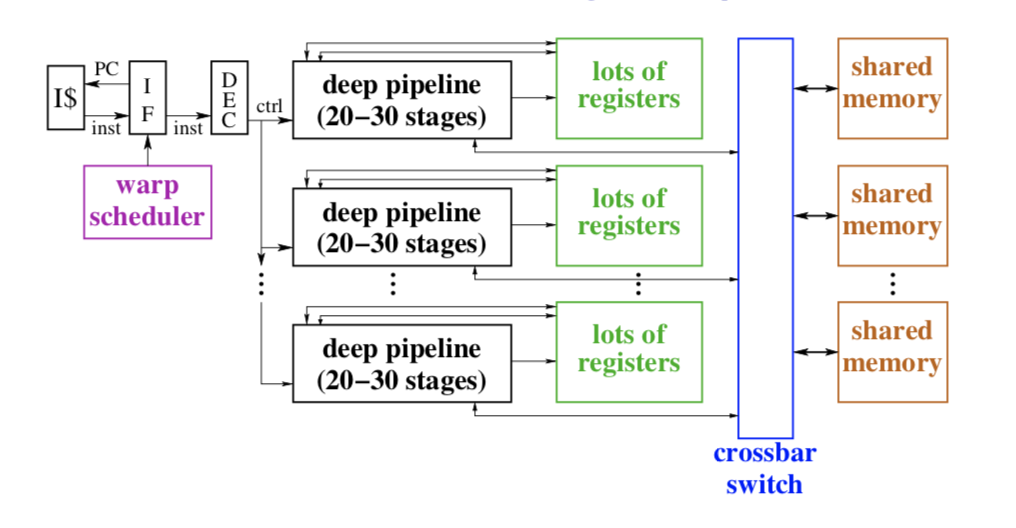
\includegraphics[scale=0.35]{images/GPU.png}
\end{center}

\begin{itemize}
	\item GPUs designed for data-parallel computing, numerical computation.
	\item GPUs are better than CPUs because they amortized the overhead of instruction fetch, decode, and pipeline control across many execution units.
	\item GPUs have higher main-memory bandwidth than CPUs because GDDR is faster than DDR.
	\item \textbf{CPUs} benefit from multiple threads so that one thread can execute while another is blocked due to a cache miss.
	\item GPUs are \textbf{Single-Instruction, Multiple-Data(SIMD)} machines
	      \begin{itemize}
		      \item Each instruction is executed for many data streams using many pipelines to hide latency
		      \item Deep pipelines: breaking instruction \textbf{execution} into small steps allows simple hardware to get good performance. More time per operation means less energy, latency is high, the throughout remains one instruction per cycle per pipeline
		      \item This amortized the cost of instruction fetch, decode, and control
		      \item The lock-step execution of the pipelines simplifies synchronization issues
		      \item No bypasses, With so many pipeline stages, bypassing become impractical. Each instruction must go all the way through the pipeline before another instruction can use the results.
	      \end{itemize}
	\item Memory
	      \begin{itemize}
		      \item Memory accesses are a major bottleneck
		      \item Caches are poor choice: one miss stalls all threads in a warp, so use \textbf{shared memory}
	      \end{itemize}
	\item Energy
	      \begin{itemize}
		      \item x86: energy goes to instruction fetch, decode and other control issues, energy for ALU operations is negligible.
		      \item GPUs: Register files are large, register file read and writes dominate the energy budget, about 10\(\times\) more energy efficient than the x86, energy for ALU operations is negligible.
	      \end{itemize}
	\item Why GPU need thousands of active threads to fully utilize the processors?
	      \begin{itemize}
		      \item \texttt{Mitigating data hazards:} Using lots of threads allows the SPs to have deep pipelines(easier to implement, lower power, higher clock speeds) without the complications of bypasses.
		            \begin{itemize}
			            \item A pipeline bypass is a mechanism that allows a result that is in the pipeline from an earlier issued instruction to be made available to a later issued instruction, even if the first instruction is still in the pipeline. Bypasses are energy hogs.
		            \end{itemize}
		      \item \texttt{Mitigating control hazards:} Even though a branch instruction takes 10s of cycles on a GPU, the SM can fetch from other warps until the branch is resolved.
		      \item \texttt{Hiding global memory latency:} Accesses to global memory are slow. Other warps can execute while a warp is waiting for a load to finish.
		      \item \texttt{Warps have lots of threads:} This amortizes the hardware, and especially the power consumption for instruction fetch, decode, and other pipeline control issues across many SPs.
		      \item \texttt{A GPU has lots of SMs:} This is how it gets lots of parallelism. But many SMs times many warps per SM times many threads per warp results in needing thousands of threads to get high performance from GPU.
	      \end{itemize}
\end{itemize}

\subsubsection{Grids, Blocks, Threads and Warps}

\begin{itemize}
	\item A \textbf{grid} is organized as an array of blocks.
	\item Each \textbf{block} is an array of threads, a block must have all execution resources it needs before it is launched
	      \begin{itemize}
		      \item A block runs on a single SM.
	      \end{itemize}
	\item \texttt{blockDim} gives the number of threads in a block, in the particular direction
	\item \texttt{gridDim} gives the number of blocks in a grid, in the particular direction
	\item \texttt{blockIdx} gives the indices of the thread's block within the grid
	\item \texttt{threadIdx} gives the indices of the thread within its block
	\item A group of thread that execute together, on each pipeline of a SIMD core are called a \textbf{warp}.
	      %   \begin{itemize}
	      %       \item \textbf{Thread divergence} is an issue when different threads in the same warp follow different control paths. If different thread execute different paths in an if-then-else, then the else-threads stall while the then-threads execute and vice verse.
	      %   \end{itemize}
	\item The \texttt{warp scheduler} determines which instruction to dispatch next instruction.
	      \begin{itemize}
		      \item If the dependencies for the next instruction are resolved, it can execute for all thread of the warp.
		      \item The hardware in each streaming multiprocessor dispatches an instruction each block cycle if a ready instruction is available.
	      \end{itemize}
\end{itemize}

% \subsubsection{Streaming Multiprocessor(SM) and Streaming Processor(SP)}

% \begin{itemize}
%     \item Each of the pipelines is a SP.
%     \item Registers and shared memory let us use a value many times without going to the off-chip, GDDR memory.
% \end{itemize}

\subsection{CUDA}

\begin{itemize}
	\item A CUDA program consists of three kinds of functions:
	      \begin{itemize}
		      \item {\textbf{\code{\_\_host\_\_} functions:} callable from code running on the host not the GPU, execute on the host CPU}
		      \item {\textbf{\code{\_\_device\_\_} functions:} callable from running on the GPU, but not the host, execute on the GPU}
		      \item {\textbf{\code{\_\_global\_\_} functions:} called by code running on the host CPU, execute on the GPU}
	      \end{itemize}
	\item Execution Model: Memory
	      \begin{itemize}
		      \item \textbf{Host Memory:} DRAM and the CPU's caches, accessible to host CPU but not to GPU.
		      \item \textbf{Device Memory:} GDDR DRAM on the graphics card, accessible by GPU, the host can initiate transfer between host memory and device memory. \textit{BUT} host cannot read/write the device memory directly.
	      \end{itemize}
	\item One or more host functions, including \code{main} to run on the host CPU.
	      \begin{itemize}
		      \item Allocate device memory.
		      \item Copy data from host memory to device memory.
		      \item Launch the device kernel by calling \code{\_\_global\_\_} function.
		            \begin{itemize}
			            \item Data parallel code that runs on the GPU is called a \textbf{kernel}.
			            \item Invoking a GPU kernel is called \textbf{launching} the kernel.
		            \end{itemize}
		            \begin{lstlisting}[language=c]
    int main(void) {
        ...
        float a = 3.0;
        saxpy<<<ceil(n/256.0),256>>>(n, a, dev x, dev y); // create n / 256 blocks, each blocks have 256 threads
        cudaMemcpy(yy, dev y, size, cudaMemcpyDeviceToHost); 
        ...
    }
                    \end{lstlisting}
		      \item Copy the result from device memory to host memory.
	      \end{itemize}
	\item \code{\_\_syncthread()}: all the threads in the block must execute this statement before any continue beyond it, all threads in the block must meet at the barrier and they must meet at the same barrier.
	\item To get good performance:
	      \begin{itemize}
		      \item perform many operations for each value copied between memories
		      \item perform many operations in the GPU fro each access to global memory
		      \item enough thread to keep the GPU cores busy
	      \end{itemize}
\end{itemize}

\subsection{CUDA Memory}

\begin{center}
	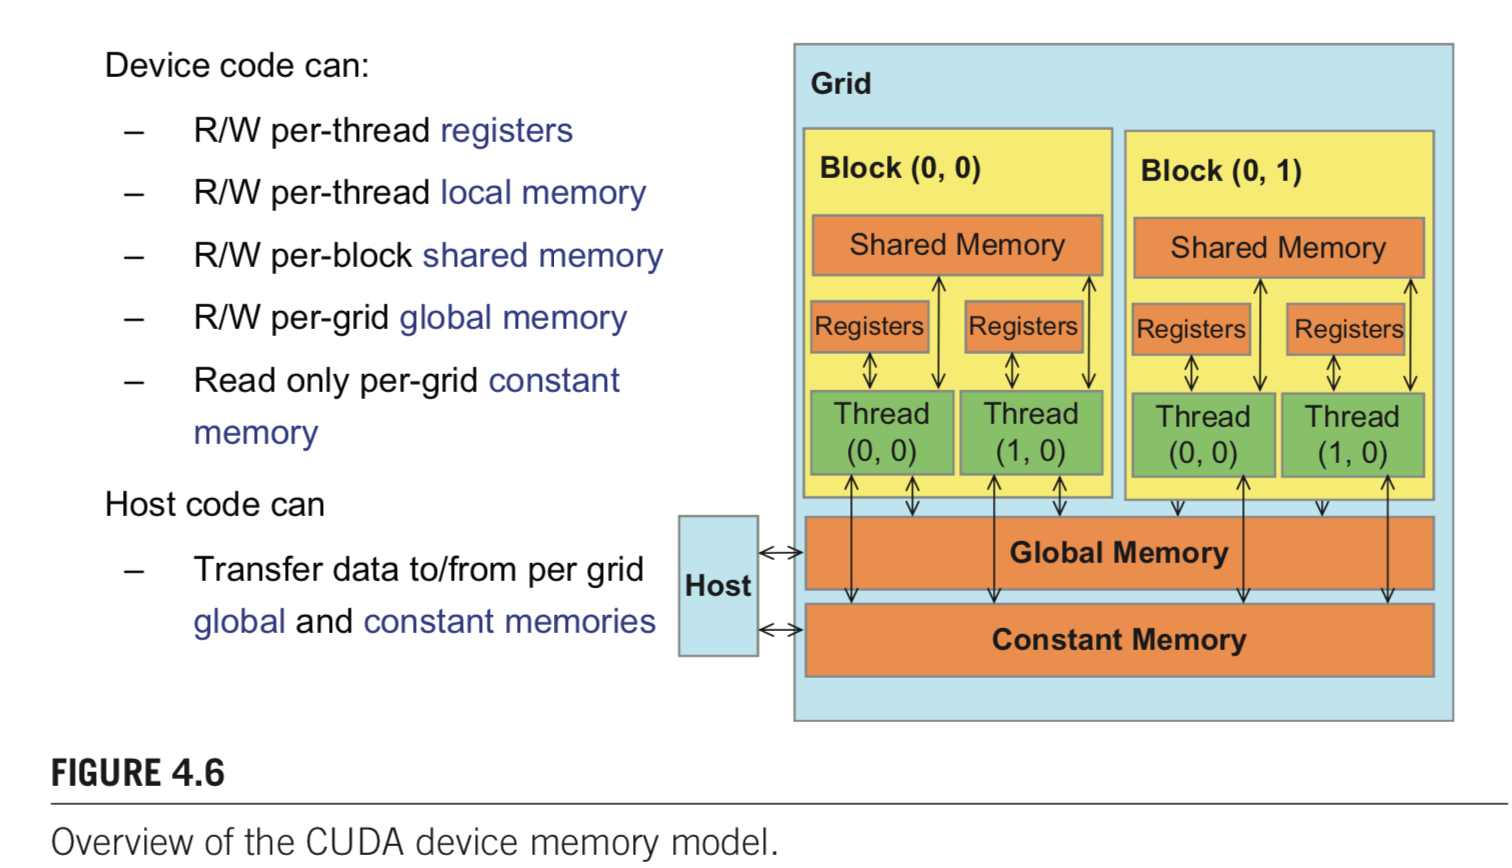
\includegraphics[scale=0.4]{images/memory.png}
\end{center}

\begin{itemize}
	\item \textbf{Registers}
	      \begin{center}
		      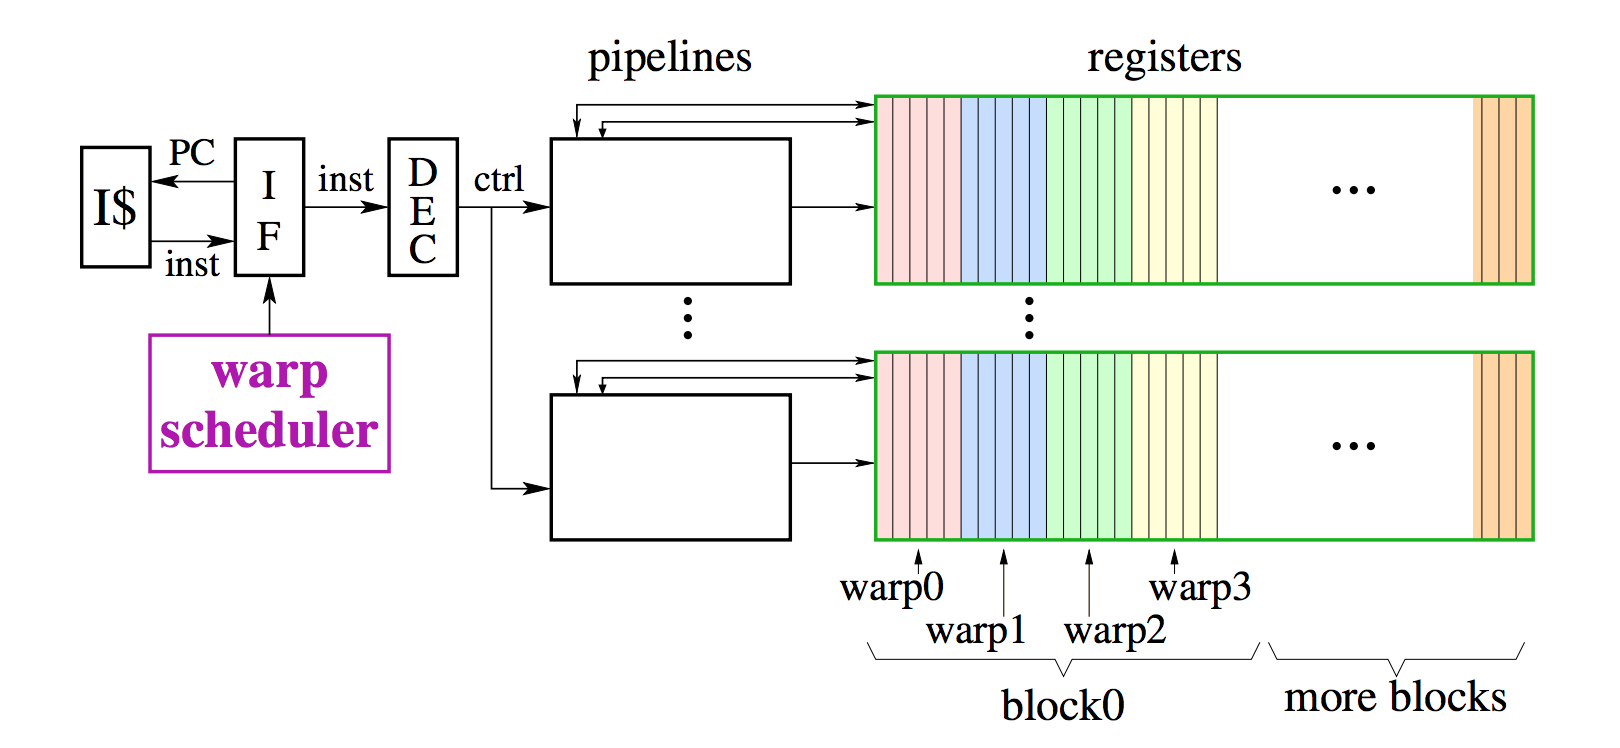
\includegraphics[scale=0.25]{images/register.png}
	      \end{center}
	      \begin{itemize}
		      \item Each SP(pipeline) has its own register file
		      \item The register file is partitioned between threads executing on the SP (32 4-byte registers per thread)
		      \item Local variables are placed in registers
		      \item in recent CUDA, threads in the same warp can swap registers
		      \item Performance trade-off:
		            \begin{itemize}
			            \item A thread can avoid slow, global memory accesses by keeping data in registers
			            \item But using too much registers reduces the number of threads that can run at the same time.
			            \item % Each CUDA device offers limited resources, thereby limiting the number of threads that can simultaneously reside in the SM for a given application. 
			                  In general, the more resources each thread requires, the fewer the threads that can reside in each SM, and likewise, the fewer the threads that can run in parallel in the entire device. % pp.97
			            \item if a thread use more registers, register will spill to main memory % FIXME: the SM cannot fully use its warp scheduler
		            \end{itemize}
	      \end{itemize}
	\item \textbf{Shared Memory}
	      \begin{itemize}
		      \item On-chip, the shared memory for each SM is partitioned into \textbf{banks}
		      \item allocated to a block, all threads in a block access the same memory
		      \item Shared memory is a limited resource (48 to 96 KBytes/SM, whereas Registers 256 Kbytes/SM)
		      \item There is a crossbar controlling the access, one thread accesses one bank at a time (90\% true)
		      \item For the GPUs we have used, there are 32 banks, selected by bits 3 through 7 of the address. This means that consecutive floats are stored in different banks. More generally, if two floats have indices that are different modulo 32, they will be in different banks.
		      \item A \textbf{bank collision} occurs if two or more threads access \textbf{different locations} belonging to the same bank and threads need to access the bank one by one.
		      \item BUT if multiple threads accesses the \textbf{same location} in the same bank, there is \textbf{no collision} because threads in the same warp can swap register, directly copy from the first thread  % FIXME:
		      \item \textbf{CON:} In general, bank conflicts are undesirable because they cause the code to run slower. References to different banks can be handled in the same clock cycle, but references to different locations in the same bank must be handled on sequentially clock cycles. Thus, conflicts increase the number of clock cycles needed to complete a load or store operation.
	      \end{itemize}
	\item \textbf{Global Memory}
	      \begin{itemize}
		      \item Off-chip DRAM
		            \begin{itemize}
			            \item when we read a location, we get 1 bit from each tile that is accessed, but we had 1024 bits available from each tile => use threads to access it coalesced % FIXME: ?????
		            \end{itemize}
		      \item The memory is mounted on DIMMs. A DIMM typically has 16 / 18 chips
		      \item Each chip consists of many "tiles", a typical chip have 4096 tiles
		      \item Each tile is an array of capacitors, a typical tile could have 1024 \(\times\) 1024 capacitors
		      \item Each capacitor holds 1 bit
		      \item Writing: easy, Reading: hard % TODO: what???
		      \item Terrible latency, fairly high bandwidth % FIXME:
		            % \item If the loads from a warp access consecutive locations, we say that the memory accesses are \textbf{coalesced}.
	      \end{itemize}

	      \begin{itemize}
		      \item \textbf{CGMA} stands for "Compute to Global Memory Access ratio"
		            \begin{align*}
			            \text{CGMA} = \frac{\# \text{FloatingPointOperations}}{\# \text{GlobalMemoryAccess}}
		            \end{align*}
		      \item CGMA for GPU: Global memory bandwidth can easily be a performance bottleneck for GPU computations. To fully utilize the computing capabilities of a GPU, we need algorithms that perform a fairly large number of operations on each data value read from or written to the global memory. The CGMA describes this ratio of the amount of computation to the number of memory references. In general, higher values for CGMA are better as code with a higher value will usually have less performance loss from memory bandwidth constraints.
		      \item CGMA for CPU: CPUs can execute a hundred instructions or more in the time that it takes to perform on DRAM access. For CPUs, the usual solution is caches. To get good performance, the average line loaded into a cache must be accessed a large number of times before it is replaced by another line from the DRAM.
	      \end{itemize}
	\item Other Memory
	      \begin{itemize}
		      \item Constant memory: caches, read-only access of global memory
		      \item Texture memory: global memory with special access operations
		      \item L1 and L2 caches: only for memory reads
	      \end{itemize}
	\item Summary
	      \begin{itemize}
		      \item GPUs can have thousands of execution units, but only a few off-chip memory interfaces
		            \begin{itemize}
			            \item which means the CPU can perform 10-50 floating point operations per every memory read or write
			            \item Arithmetic operations are very cheap compared with memory operations
		            \end{itemize}
		      \item Use Registers and the per-block shared memory to mitigate the off-chip memory bottleneck
		      \item Moving data between different kinds of storage is the programmer's responsibility
	      \end{itemize}

\end{itemize}

\subsection{CUDA Performance Considerations}

\begin{itemize}
	\item Floating Point Foibles
	      \begin{itemize}
		      \item GPUs are optimized for single precision floating point arithmetic
		      \item if one operands is double precision, the compilations done using double precision arithmetic
		      \item A \textbf{fused multiply-add}, a common fracture in hardware for floating-point arithmetic where a multiply followed by an add, e.g.,\(a * X + b\), can be computed as a single operation. But it counts as 2 floating point operations.
	      \end{itemize}
	\item Shared Memory Accesses faster than global memory, but watch out shared-memory bank conflicts
	\item Global Memory Accesses
	      \begin{itemize}
		      \item \textbf{Coalescing references:} If the threads of a warp access consecutive locations of the global memory, the memory reference is said to be coalesced. Coalesced memory references only make one global memory access.
		      \item \textbf{PRO:} The GPU can take advantage of accessing a large, contiguous block of memory and achieve high bandwidth with the data transfer. Conversely, if locations are not coalesced, then several bank accesses may be needed, and several transfers of data from the DRAM to the GPU. Thus, coalesced references are handled faster than non-coalesced ones.
		      \item coalesced accesses to global memory are faster than worst-case bank collision with the shared memory
	      \end{itemize}
	\item SMs and Thread Occupancy
	      \begin{align*}
		      \text{threadOccupancy} \leq \min(8, \lfloor \frac{2048}{\text{threadsPerBlock}}\rfloor) \times \frac{2048}{\text{threadsPerBlock}}
	      \end{align*}
	      \begin{itemize}
		      \item An SM has warps of 32 threads.
		      \item An SM can simultaneously execute up to 2048 threads (64 warps).
		      \item An SM can simultaneously execute up to \(\min (8,\lfloor 2048 / \text{threadsPerBlock} \rfloor)\) blocks.
		      \item An SM has 96K bytes of shared memory.
		      \item An SM has 64K (\(2^{16}\)) 32-bit registers (1K registers/SP).
		      \item Each block can have up to 1024 threads, we want at least \textbf{2} blocks per SM, more is better.
		      \item Each block can have up to 48K bytes of shared memory.
	      \end{itemize}
	\item Instruction Mix, the program does other operations as well, so optimizing performance can involve minimizing this overhead
	      \begin{itemize}
		      \item Good algorithm design
		      \item Memory access optimization
		      \item Bigger Kernels: when \code{do something} is big, kernel launch takes most the time.
		      \item Loop Unrolling: two or three instruction per loop iteration to manage the loop, so each loop iteration perform multiple copies of the loop body
	      \end{itemize}
	\item \textbf{Thread divergence} occurs when different threads in the same warp follow different execution paths. For example, one executes the “then-”clause” of an if-statement and the other executes the “else”.
	      \begin{itemize}
		      \item \textbf{CON:} Thread divergence is undesirable because the GPU must execute both paths, and only some of the pipelines are active for each path. This results in idle execution pipelines.
		      \item It can be worse,
		            \begin{itemize}
			            \item Nested if-then-else statements, divide threads into more than two groups
			            \item For-loops with thread-dependent bounds, while-loops
		            \end{itemize}
		      \item It can be better,
		            \begin{itemize}
			            \item If all threads in a warp are then-threads, then the else-instructions aren't fetched, vice verse.
		            \end{itemize}
		      \item \code{\_\_syncthreads()} implements a barrier: all threads in the block must reach the barrier before any continue beyond it.
		            \begin{itemize}
			            \item e.g. \code{\_\_syncthreads()} in a then-clause for one thread can't match a \code{\_\_syncthreads()} in a else-clause for another thread. \textbf{deadlock:} the block hangs forever at the \code{\_\_syncthreads()}
			            \item If there is a \code{\_\_syncthreads()} in the body of a for-loop, all threads must reach it on the same iteration.
		            \end{itemize}
	      \end{itemize}
\end{itemize}

\end{document}
